\documentclass[a4paper,12pt]{article}
\usepackage[a4paper,top=1.3cm,bottom=2cm,left=1.5cm,right=1.5cm,marginparwidth=0.75cm]{geometry}
\usepackage{setspace}
\usepackage{cmap}					
\usepackage{mathtext} 				
\usepackage[T2A]{fontenc}			
\usepackage[utf8]{inputenc}			
\usepackage[english,russian]{babel}
\usepackage{multirow}
\usepackage{graphicx}
\usepackage{wrapfig}
\usepackage{tabularx}
\usepackage{float}
\usepackage{longtable}
\usepackage{hyperref}
\hypersetup{colorlinks=true,urlcolor=blue}
\usepackage[rgb]{xcolor}
\usepackage{amsmath,amsfonts,amssymb,amsthm,mathtools} 
\usepackage{icomma} 
\mathtoolsset{showonlyrefs=true}
\usepackage{euscript}
\usepackage{mathrsfs}
\DeclareMathOperator{\sgn}{\mathop{sgn}}
\newcommand*{\hm}[1]{#1\nobreak\discretionary{}
	
	{\hbox{$\mathsurround=0pt #1$}}{}}


\begin{document}
	\begin{titlepage}
		\begin{center}
			{\large МОСКОВСКИЙ ФИЗИКО-ТЕХНИЧЕСКИЙ ИНСТИТУТ (НАЦИОНАЛЬНЫЙ ИССЛЕДОВАТЕЛЬСКИЙ УНИВЕРСИТЕТ)}
		\end{center}
		\begin{center}
			{\large Физтех-школа физики и исследований им. Ландау}
		\end{center}
		
		
		\vspace{4.5cm}
		{\huge
			\begin{center}
				{\bf Отчёт \\ Лабораторная работа 1.2.5}\\
				Исследование прецессии уравновешенного гироскопа 
			\end{center}
		}
		\vspace{2cm}
		\begin{flushright}
			{\LARGE Третьяков Александр\\
				\vspace{0.2cm}
				Б02-206}
		\end{flushright}
		\vspace{8cm}
	\end{titlepage}
	
	\section{Введение}
	
	\textbf{Цель работы:} исследовать вынужденную прецессию гироскопа; установить зависимость скорости вынужденной прецессии от величины момента сил, действующих на ось гироскопа; определить скорость вращения ротора гироскопа и сравнить ее со скоростью, рассчитанной по скорости прецессии\\
	\textbf{Оборудование:} гироскоп в кардановом подвесе, секундомер, набор грузов, отдельный ротор гироскопа, цилиндр известной массы, крутильный маятник, штангенциркуль, линейка.
	
	\section{Теоретические сведения}
	В данной работе исследуется регулярная прецессия уравновешенного гироскопа.//
	В первой части работы исследуется зависимость скорости прецессии гироскопа от момента силы, приложенной к его оси. Для этого к оси гироскопа (к рычагу С) подвешиваются грузы Г. Скорость прецессии определяется по числу оборотов рычага вокруг вертикальной оси и времени, которое на это ушло, определяемому секундомером. В процессе измерений рычаг не только поворачивается в результате прецессии гироскопа, но и опускается. Поэтому его в начале опыта следует преподнять на $5-6^{\circ}$. Опыт нужно закончить, когда рычаг опустится на такой же угол.\\
	\begin{center}$
		\begin{array}{cc}
			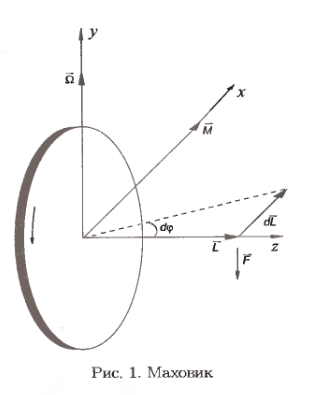
\includegraphics[width=0.40\textwidth]{img1.png}&
			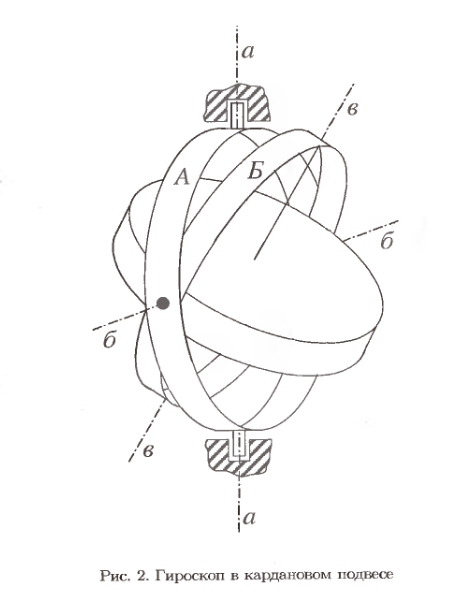
\includegraphics[width=0.40\textwidth]{img2.png}\\
		\end{array}$
	\end{center}
	
	Измерение скорости прецессии гироскопа позволяет вычислить угловую скорость вращения его ротора. Расчет производится по формуле:
	
	\begin{equation}
		\Omega = \frac{mgl}{I_z\omega_0},
	\end{equation}
	
	где $m$ -- масса груза, $l$ -- расстояние от центра карданова подвеса до точки крепления груза на оси гироскопа (рис. 3), $I_z$ -- момент инерции гироскопа по его главной оси вращения. $\omega_0$ -- частота его вращения относительно главной оси, $\Omega$ -- частота прецессии.\\
	Момент инерции ротора относительно оси симметрии $I_0$ измеряется по крутильным колебаниям точной копии ротора, подвешиваемой вдоль оси симметрии на десткой проволоке. Период крутильных колебаний $T_0$ зависит от момента инерции $I_0$ и модуля кручения проволоки $f$:
	
	\begin{equation}
		T_0 = 2\pi\sqrt{\frac{I_0}{f}}.
	\end{equation}
	
	Чтобы исключить модуль кручения проволоки, вместо ротора гироскопа к той же проволоке подвешивают цилиндр правильной формы с известными размерами и массой, для которого легко можно вычислить момент инерции $I_\text{ц}$. Для определения момента инерции ротора гироскопа имеем:
	
	\begin{equation}
		I_0 = I_\text{ц}\frac{T_0^2}{T_\text{ц}^2},
		\label{moment}
	\end{equation}
	Здесь $T_\text{ц}$ -- период крутильных колебаний цилиндра.\\
	\begin{center}
		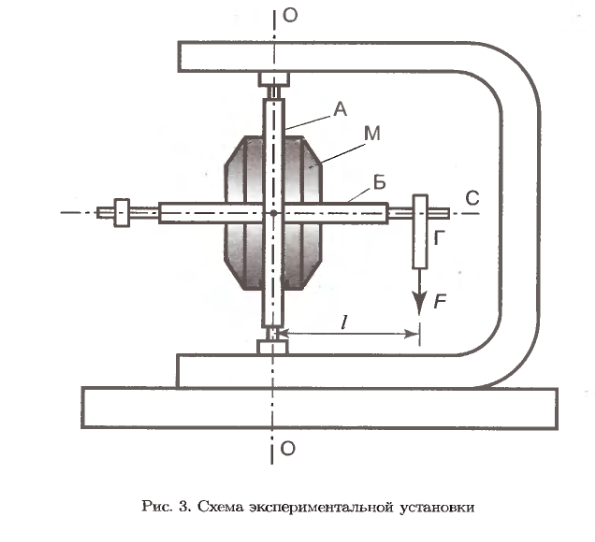
\includegraphics[width=0.8\textwidth]{img3.png}
	\end{center}
	
	Скорость вращения ротора гироскопа можно определить и не прибегая к исследованию прецессии. У используемых в работе гироскопов статор имеет две обмотки, необходимые для быстрой раскрутки гироскопа. В данной работе одну обмотку искользубт для раскрутки гироскопа, а вторую -- для измерения числа оборотов ротора. Ротор электромотора всегда немного намагничен. Вращаясь, он наводит во второй обмотке переменную электродвижущую силу(ЭДС) индукции, частота которой равна частоте врещения ротора. Частоту этой ЭДС можно, в частности, измерить по фигурам Лиссажу, получаемым на экране осциллографа, если на один вход подать исследуемую ЭДС, а на другой -- переменное напряжение с хорошо прокалиброванного генератора. При совпадении частот на эеране получаем эллипс.
	
	\section{Ход работы}
	Измеряем вместе с напарником период колебаний цилиндра ($m=1617,0$ г, $2R=78,1$ мм) с помощью ручного секундомера по три замера каждый для 5 колебаний, аналогично для ротора; плечо $l=122$:
	
	
	\begin{table}[h]
		\centering
		\begin{tabular}{|l|l|l|c|l|}
			\hline
			N & $T_\text{5цил}$ & $T_{5\text{ротор}}$ & \multicolumn{1}{l|}{$T_\text{цил}$} & $T_\text{ротор}$                \\ \hline
			5 & 21.04 & 16.00   & \multirow{6}{*}{4,1}      & \multirow{6}{*}{3,22} \\ \cline{1-3}
			5 & 20.63 & 15.88   &                           &                       \\ \cline{1-3}
			5 & 20.42 & 16.07   &                           &                       \\ \cline{1-3}
			5 & 20.70 & 16.56   &                           &                       \\ \cline{1-3}
			5 & 20.46 & 16.02   &                           &                       \\ \cline{1-3}
			5 & 20.35 & 16.10   &                           &                       \\ \hline
		\end{tabular}
	\end{table}
	Высчитаем $I_\text{г}=I_{\text{цил}}\frac{T_{\text{ротор}}^{2}}{T_{\text{цил}}^{2}}\approx 7.7\cdot 10^{-4}$ кг$\cdot\text{м}^2$. Рассмотрим погрешности, которые есть в $I_\text{г}$:
	

	\begin{equation}
		\sigma_{T_{\text{ротор}}}^\text{случ}=\sqrt{\frac{1}{n(n-1)} \sum_{i=1}^{n}(T_{\text{ротор }i} - \overline{T_{\text{ротор}}})^2}\approx 0,1 c 
	\end{equation}
	
	
	\begin{equation}
		\sigma_{T_{\text{ротор}}}^\text{сист}=0,2 c
	\end{equation}
	\begin{equation}
		\sigma_{T_{\text{цил}}}^\text{2 полн}=\sqrt{\sigma_{T_{\text{ротор}}}^\text{2 сист} + \sigma_{T_{\text{цил}}}^\text{2 случ}} = \sqrt{0,2^2 + 0,1^2}\approx 0,22 с
	\end{equation}
	
	\begin{equation}
		\varepsilon_{T_{\text{ротор}}}\approx 1,12\%
	\end{equation}
	\begin{equation}
		\varepsilon_{T_{\text{ротор}}^2}\approx 2*1,12\%=2,24\%
	\end{equation}
	
	\begin{equation}
		\varepsilon_{m\text{ц}}\ll 0.1\%
	\end{equation}
	
	\begin{equation}
		\varepsilon_{R^2}\approx 2*0,64\%=1,28\%
	\end{equation}
	
	
	Видно, что погрешность массы цилиндра можно не учитывать при расчетах, потому что она очень мала по сравнению с погрешностью измерения времени по секундомеру вручную и диаметра
	\begin{equation}
		\varepsilon_{I_\text{г}}= \sqrt{(\varepsilon_{T_{\text{ротор}}^2})^2 + (\varepsilon_{T_{\text{цилиндр}}^2})^2+ (\varepsilon_{R^2})^2} \approx 3,29\%
	\end{equation}
	Отсюда можем сделать вывод, что важно как можно точнее измерять период у ротора и цилиндра, чтобы уменьшить погрешность.
	
	Теперь посчитаем коэффициент установки $k$:
	\begin{equation}
		k=\frac{gl}{2\pi I_\text{г}}\approx 252 
	\end{equation}
	Рассмотрим погрешности, которые есть в $k$:
	
	\begin{equation}
		\varepsilon_{l}=\frac{0.5 \text{мм}}{122 \text{мм}}*100\%\approx 0,41\%
	\end{equation}
	\begin{equation}
		\varepsilon_{I_\text{г}}\approx 3,29\%
	\end{equation}
	Видим, что значительно больший вклад вносит погрешность момента инерции
	\begin{equation}
		\varepsilon_{k}=\sqrt{(\varepsilon_{l})^2 + (\varepsilon_{I_\text{г}})^2} \approx 3,32\%
	\end{equation}
	Поэтому нужно уменьшать погрешность периода.\\
	Теперь, зная коэффициент установки, будем вешать грузы массы $m$ и измерять период с помощью секундомера\\
	\begin{table}[]
		\centering
		\begin{tabular}{|l|l|l|l|l|l|l|l|l|l|l|l|}
			\hline
			$m$     & $T_{cp} $     & $\omega_{fixed}$  & $\nu_{fixed} $ & $\nu_{osc}$ & $\delta$    & $\delta_{fake}$ & $\omega$      & $\nu4$      & $k$   & $\varepsilon_{\nu}$ & $\sigma_{\nu}$ \\ \hline
			141,2 & 69,7   & 2480,093 & 394,7191 & 391   & 3,719105 & 0,951178 & 2561,1 & 407,6  & 252 & 3,34 & 13,2       \\ \hline
			112   & 89,51  & 2526,33  & 402,0779 & 391   & 11,07795 & 2,833234 & 2612,6 & 415,8  & 252 & 3,4 & 13,7     \\ \hline
			267   & 37,93  & 2552,082 & 406,1765 & 392   & 14,17648 & 3,61645  & 2639,4 & 421,1  & 252 & 3,43 & 13,9      \\ \hline
			93    & 107,58 & 2521,245 & 401,2686 & 391   & 10,26859 & 2,626237 & 2607,3 & 415    & 252 & 3,34 & 13,4      \\ \hline
			215   & 46,1   & 2497,698 & 397,521  & 390   & 7,520983 & 1,928457 & 2583,7 & 411,21 & 252 & 3,38 & 17,4     \\ \hline
		\end{tabular}
	\end{table}
	
	Столбец $\omega_{fixed}$ - после исправления ошибки в измерениях коэффициента установки $k$(столбец $\omega$ - до исправления)
	Теперь посчитаем погрешность омеги $\omega_{fixed} = kmT $ в эксперименте. Погрешность массы грузов не будем учитывать, потому что она очень мала по сравнению с погрешностью коэффициента установки.
	\begin{equation}
		\sigma_{T_{\text{ср}}}^\text{сист}=0,2 c
	\end{equation}
	\begin{equation}
		\sigma_{T}^\text{случ}=\sqrt{\frac{1}{n(n-1)} \sum_{i=1}^{n}(T_{i} - \overline{T)^2}}\approx 0,2 c
	\end{equation}
	
	\begin{equation}
		\sigma_{T}^\text{полн}=\sqrt{\sigma_{T}^\text{2 сист} + \sigma_{T}^\text{2 случ}} = \sqrt{0,2^2 + 0,2^2}\approx 0,28 c
	\end{equation}
	
	\begin{equation}
		\varepsilon_{T_\text{ср}}= 0,4\%
	\end{equation}
	
	\begin{equation}
		\varepsilon_{\omega_\text{fixed1}}= \sqrt{(\varepsilon_{T_{cp}})^2 + (\varepsilon_{k})^2} \approx 3,34\% = \varepsilon_{\nu_\text{fixed1}}
	\end{equation}
	Относительные погрешности совпадают, потому что $\omega = 2\pi\nu$
	\begin{equation}
		\sigma_{\nu\text{fixed1}}=  \varepsilon_{\nu\text{fixed1}} * \nu_\text{fixed1} = 394,7\cdot3,3/100  = 13 \text{ Гц}
	\end{equation}
	Можем заметить, что здесь измерения периода вносят в погрешность меньше, чем k, потому что измеряемые промежутки времени больше, чем при измерении цилиндра. Посчитаем погрешности и внесем их в таблицу. \\
	%Тогда мы получим такие значения с учетом погрешностей:
	%  \begin{itemize}
		%%		\item $\nu = (394,7 \pm 13,2)\text{ Гц } (\varepsilon_\nu = 3,34\%)$ 
		%%		\item $\nu = (402,1 \pm 13,7)\text{ Гц } (\varepsilon_\nu = 3,4\%)$ 
		%%		\item $\nu = (406,2 \pm 13,9)\text{ Гц } (\varepsilon_\nu = 3,43\%)$ 
		%		\item $\nu = (401,3 \pm 13,4)\text{ Гц } (\varepsilon_\nu = 3,34\%)$ 
		%		\item $\nu = (397,5 \pm 17,4)\text{ Гц } (\varepsilon_\nu = 3,38\%)$ 
		%	\end{itemize}
	В целом все погрешности примерно равны 3,4\%, поэтому можем сказать, что мы в итоге получили $\nu =  400,35 \pm 13,62 \text{ Гц} (\varepsilon_\nu = 3,4\%)$, это попадает в значение $\nu_{\text{осц}}=391 \text{ Гц}$, полученное с помощью осциллографа
	
	\section{Оценка момента силы трения}
	
	Оценим момент силы трения, действующей на ось гироскопа
	
	\
	$$T =\frac{360^\circ}{\Delta \alpha} t = \frac{360}{15}  240 c \eqsim 5760 c$$
	По полученным данным мы можем оценить момент силы трения, действующей на ось гироскопа по следующей формуле:
	
	Оценить момент силы трения мы можем по формуле: $M = \frac{2\pi}{T}I_{\text{г}} \omega$, а $\sigma_M = M\cdot\sqrt{\varepsilon_M^2+ \varepsilon_k^2}$. Для каждой массы момент силы трения будет свой, но мы оценили только для одной массы:
	
	\begin{itemize}
		\item $m = 215$ г, $\omega = 2498$ $\text{с}^{-1}$, $M = (2,10\pm0,02)\cdot10^{-3}$ Н$\cdot$м
	\end{itemize}  
	Видим, что он оказывается достаточно мал по сравнению с моментом силы тяжести груза, подвешенного на ось гироскопа, но его хватает для поворота гироскопа
	
	\section{Обсуждение результатов и выводы}
	
	В ходе работы мы определили частоту вращения ротора гироскопа:
	
	\begin{itemize}
		\item \underline{$ \nu = \left( 400,35 \pm 13,62 \right) \text{ Гц}, \left( \varepsilon = 3,4 \% \right)   $}
	\end{itemize}
	Если учесть погрешность, то частота совпадет со значением частоты, которую получили с помощью осциллографа ($ \nu_\text{осц} = 391 $ Гц)\\
	Уменьшить погрешность частоты можно, если точнее измерить период колебаний цилиндра и ротора, потому что они дают самую большую погрешность в коэффициент установки, который потом влияет на все дальнейшие расчеты.\\
	Еще мы оценили момент силы трения, действующий на ось гироскопа $M = (2,10\pm0,02)\cdot10^{-3} H$. Он получился мал, если сравнивать с моментом силы тяжести груза, но его все равно хватает для поворота гироскопа в сторону направления силы тяжести груза. Чтобы оценить его точнее, нужна хорошая шкала определения отклонения угла, но у нас такой не было, пришлось определять отклонение на глаз и линейку.
	
	
	
	
\end{document}